\author{Mudith Witharama}
\documentclass[a4paper,12pt]{article}
\usepackage{subcaption}
\usepackage{ragged2e}
\usepackage{float}
\usepackage{titlesec}
\usepackage[english]{babel}
\usepackage[nottoc]{tocbibind}% use references in table of content
%\usepackage{hyperref}
\usepackage[colorlinks=true,plainpages=true,citecolor=blue,linkcolor=blue]{hyperref}
\usepackage{amsmath}
\usepackage{longtable}
\usepackage{float}
\usepackage{booktabs}
\usepackage[toc,page]{appendix}
% \usepackage{acro}
\usepackage[utf8]{inputenc}
\usepackage[acronym, toc]{glossaries}

% probably a good idea for the nomenclature entries:
% \acsetup{first-style=short}

\titleclass{\subsubsubsection}{straight}[\subsection]
\newcounter{subsubsubsection}[subsubsection]
\renewcommand\thesubsubsubsection{\thesubsubsection.\arabic{subsubsubsection}}
\renewcommand\theparagraph{\thesubsubsubsection.\arabic{paragraph}} % optional; useful if paragraphs are to be numbered

\titleformat{\subsubsubsection}
  {\normalfont\normalsize\bfseries}{\thesubsubsubsection}{1em}{}
\titlespacing*{\subsubsubsection}
{0pt}{3.25ex plus 1ex minus .2ex}{1.5ex plus .2ex}
\title{\Large Exploring Graph Neural Networks in Optimal Power Flow Problem} 

\makeatletter
\renewcommand\paragraph{\@startsection{paragraph}{5}{\z@}%
  {3.25ex \@plus1ex \@minus.2ex}%
  {-1em}%
  {\normalfont\normalsize\bfseries}}
\renewcommand\subparagraph{\@startsection{subparagraph}{6}{\parindent}%
  {3.25ex \@plus1ex \@minus .2ex}%
  {-1em}%
  {\normalfont\normalsize\bfseries}}
\def\toclevel@subsubsubsection{4}
\def\toclevel@paragraph{5}
\def\toclevel@paragraph{6}
\def\l@subsubsubsection{\@dottedtocline{4}{7em}{4em}}
\def\l@paragraph{\@dottedtocline{5}{10em}{5em}}
\def\l@subparagraph{\@dottedtocline{6}{14em}{6em}}
\let\thetitle\@title % added by kithmini
\makeatother

\setcounter{secnumdepth}{4}
\setcounter{tocdepth}{4}

\usepackage[utf8]{inputenc}
\usepackage[english]{babel}
\usepackage[top=1in, bottom=1in, left=1in, right=1in]{geometry}
\usepackage{fancyhdr}
\pagestyle{fancy}
\fancyhf{}
\rhead{EE3203}
\lhead{Individual Project}
\cfoot{\thepage}
\usepackage{graphicx}
% \usepackage{biblatex}

\graphicspath{{Images/}}

%to embed code
\usepackage{listings}
\newsavebox{\mybox}
\usepackage{color} %red, green, blue, yellow, cyan, magenta, black, white
\definecolor{mygreen}{RGB}{28,172,0} % color values Red, Green, Blue
\definecolor{mylilas}{RGB}{170,55,241}

\lstset{
  language=Matlab,%
    basicstyle={\small\ttfamily},
    breaklines=true,%
    morekeywords={matlab2tikz},
    keywordstyle=\color{blue},%
    morekeywords=[2]{1}, keywordstyle=[2]{\color{black}},
    identifierstyle=\color{black},%
    stringstyle=\color{mylilas},
    commentstyle=\color{mygreen},%
    showstringspaces=false,%without this there will be a symbol in the places where there is a space
    rulecolor=\color{black},
    numbers=left,%
    numberstyle={\tiny \color{black}},% size of the numbers
    numbersep=9pt, % this defines how far the numbers are from the text
    emph=[1]{for,end,break},emphstyle=[1]\color{blue}, %some words to emphasise
    tabsize=3,
    xleftmargin=2em,
    frame=single,
    framexleftmargin=1.5em
    %emph=[2]{word1,word2}, emphstyle=[2]{style}, 
}

\makeglossaries

\newacronym{opf}{OPF}{Optimal Power Flow}
\newacronym{gnn}{GNN}{Graph Neural Network}
\newacronym{ipopt}{IPOPT}{Interior Point Optimization Technique}
\newacronym{pp}{PP}{Power Plant}
\newacronym{ai}{AI}{Artificial Inteligence}

\begin{document}

\begin{titlepage}
\newcommand{\HRule}{\rule{\linewidth}{0.5mm}}
\center
\textsc{\small DEPARTMENT OF ELECTRICAL ENGINEERING\\}
	\textsc{\small UNIVERSITY OF MORATUWA}\\[1.0 cm]
    \vspace*{0.5 cm}

\vspace{\baselineskip} 
\vspace{\baselineskip} 

\textsc{\large EE3203 - Individual Project}\\[0.8cm]


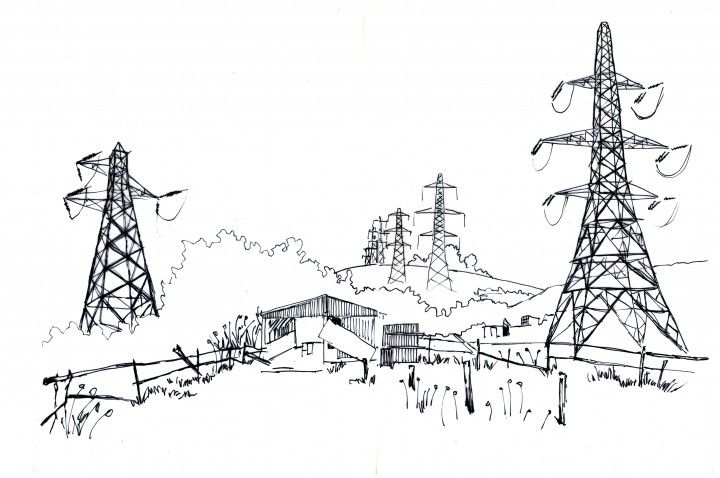
\includegraphics[scale = 0.4]{Images/drawing_line.jpg}\\[1cm]
\vspace{\baselineskip} 
{ \huge \bfseries \thetitle}\\
\HRule \\[1.0cm]

%\flushcenter 
\Large
\vspace{\baselineskip} 
\vspace{\baselineskip} 
\vspace{\baselineskip} 
\begin{minipage}{0.4\textwidth}
		\begin{flushleft}
			W. M. N. Witharama
			\end{flushleft}
			\end{minipage}
			\begin{minipage}{0.1\textwidth}
			\begin{flushright}
			(180719L)
		\end{flushright}
	\end{minipage}\\[1 cm]
	 {\small \textit{This report is submitted for the module EE3203}}\\[0.2 cm]
	 ---\\

\center {\today}
\vfill 
\end{titlepage}
\newpage
% Do not edit the below sections, enter all details in respective chapters
% Add the images/screen-shorts to the image folder and insert them in the respective chapters

\tableofcontents

\newpage
\listoffigures

\newpage
\printglossary[type=\acronymtype]


\pagebreak
\section{Introduction}
\subsection{Background}
With the increase in fuel prices and the increasing demand for energy, the cost of energy generation is continuously rising. This total cost is an important factor in providing electricity to consumers at a reasonable price.

 Due to the environmental concerns of fossil fuel-based energy generation, renewable energy sources are getting popular. But this has its own challenges when it comes to the power grid. This adds lots of distributed generators making it difficult to maintain the balance of the grid while minimizing the total generation cost in future power systems.  \\
\\  \hyperref[sec:opfIdentify]{Optimal Power Flow}, is the minimization of the total generating cost of a power system by determining the optimal amount of power required to generate at each power plant. 


\subsection{Motivation}

Traditional power grids were centralized making it simple to decide the power generation required from each power plant. As more power plants are introduced to the grid, several approaches have been researched to find a solution to this Optimal Power Flow problem. \\

\acrlong{gnn} is a novel concept that has outperformed traditional neural network-based and artificial intelligence-based algorithms in graph and node classification problems, graph clustering applications, etc.\\

A Power System can be considered as a graph where nodes resemble buses and edges resemble transmission lines.  D.Owerko, F.Gama and A. Ribeiro have published a paper Optimal Power Flow Using Graph Neural Networks\cite{Owerko2020OptimalNetworks} attempting to apply this novel \acrshort{gnn} model to the optimal power flow problem. Since their experiments have promising results for a basic Graph Neural Network with two hidden layers I intend to further explore this area.

\subsection{Optimal Power Flow Problem Identification}
\label{sec:opfIdentify}
Optimal Power Flow is determining the active and reactive power that needs to be generated by each power plant in a power grid, to reduce the total generation cost. This is one of the most important optimization problems in the energy industry \cite{Cain2012HistoryFormulations}. This history of this problem goes back a couple of decades. But still, we do not have an efficient solution for large power systems and if found, the total cost can be reduced considerably \cite{Cain2012HistoryFormulations}. \\

Different generators have different costs per unit.
One may assume that the cost is minimized if all the power is generated from the cheapest generators. But the losses in transmission lines account for the total loss and supplying the demand from nearby generators is sometimes more effective than supplying from a distant cheaper generator.\\
 
\newpage
We define the problem as follows.
Each node in the graph describes the Voltage $(v^{( i)})$,Phase angle$(\delta^{( i)})$,Active Power$(p^{( i)})$ and Reactive Power$(q^{( i)})$ consumed. We say there are N nodes, thus we can use an N*4 matrix $(X^{(N*4)})$ to store the input data as follows.\\

\[
 \begin{array}{l}
x^{( i)} \ =\ \left[ v^{( i)} \ \delta ^{( i)} \ p^{( i)} \ q^{( i)}\right]
\end{array}
\]

\[
 \begin{array}{l}
 X^{N*4}
\end{array}
\]

$x^{(i)}$ describes the features of one node and matrix X describes  $x^{(i)}$ features of all nodes. Objective of this problem is to minimize the cost per unit time defined by,


\[ \sum_{n=1}^{G} C_{m}( P_{m}) \]

Here $C$ is the cost function of $m^{th}$ generator and G is the number of generators. $P_{m}$ represents the power generated at each generator. The above equation describes the total cost.
\subsection{Research Approach}
\\IEEE 30 test case data was accessed through PandaPower\cite{Thurner2017PandapowerSystems}, Python library and then optimal solutions were calculated from Interior Point Optimization Method\cite{Wachter2006OnProgramming}, which is a slow mathematical technique, through the same PandaPower library.
Then Graph Neural Network was trained to imitate the above results for the data set.\\

Skorch was used as the Neural Network Library and the GNN library written by F.Gama was used as the Graph Neural Network library.
Different Neural Network Architectures, Optimizers and Scaling Factors were experimented.


\subsection{Objectives}


Minimizing the cost of Generation of a large power system, optimizing the parameters and calculating the optimum values of generations needed from each \acrlong{pp} is the main objective of \acrshort{opf} problem.\\
 
 I intended to study the areas of Graph Convolution and Graph Neural Network and its applications in Power Systems.\\
 
 In addition, another objective of this project is to further explore the work\cite{Owerko2020OptimalNetworks} done by D.Owerko, F. Gama and A. Ribeiro and to experiment with the parameters and analyse how the changes to the \acrlong{gnn} architecture, optimizer and scaling factor affect overall performance.
 
\newpage
\section{Literature Review}
Throughout the past decades, several approaches were experimented with to solve this \acrshort{opf} problem\cite{Cain2012HistoryFormulations}\\
\\ Some of these approaches are Mathematical Optimization techniques and their computation time is high for real-world large power systems. The quasi-Newton method, which is a mathematical method based approach was applied for this \acrshort{opf} problem\cite{Tang2017Real-TimeFlow}. This approach successfully addresses the randomness and fluctuations in future power systems. Although the mathematical methods are accurate, their convergence time is very high and not scalable beyond IEEE 30 test case. Furthermore, due to the sinusoidal nature of voltage and current, this problem is non-convex and difficult to solve.\cite{Bienstock2019StrongFeasibility}\\

Genetic Algorithms and Artificial Intelligence-based algorithms and several other algorithms were also used to solve this problem.\\

Enhanced adaptive differential evolution (JADE) with self-adaptive penalty constraint handling technique, referred to as EJADE-SP, obtain the optimal solution of the OPF problem \cite{Li2020OptimalEvolution}. This method can be used to find additional information such as real power loss, voltage deviation, emission and emission cost. But their method is not scalable and experiment results are limited to IEEE 30 test cases.\\

Small-angle approximation of trigonometric terms of voltage angle differences is widely used in industry \cite{Cain2012HistoryFormulations}. Although this approach speeds up the computation time it fails for heavily-loaded 
networks, since differences in voltage angles become large \cite{Bienstock2019StrongFeasibility} \\

Machine Learning algorithms have also been experimented with this \acrshort{opf} problem\cite{Guha2019MachineFlow}. These algorithms optimizes the cost while respecting physical and engineering constraints. In addition, nature-inspired algorithms like Sun Flower Optimization algorithm was applied to this problem with a satisfactory outcome in power systems with distributed generators \cite{Shaheen2019OptimalAlgorithm}
But some of the areas in AI are still evolving and very recent developments are not yet applied to power systems and the OPF problem.\\


Graph Neural Network\cite{Liu2020IntroductionNetworks} is a new domain in Neural Networks and \acrlong{ai}. It has a wide range of applications in chemical systems, traffic networks, recommendation systems, image processing and social network analysis\cite{Zhou2020GraphApplications}. D. Owerko, F. Gama and A. Ribeiro proved that the applications of \acrshort{gnn} extend beyond the above domains and it is applicable in power systems as well.
Although the success of previous methods were mainly limited to small power systems such as IEEE 30 test case, they proved that the \acrshort{gnn} is scalable to large power systems. The experiments on IEEE 118 proves their claim.
But their experiments are done using small two hidden layer neural networks and analysis on how the changes of neural network architecture, optimizer affects the overall results is not discussed.


\section{GNN Model}

\subsection{Machine Learning and Neural Networks}
Machine Learning is a branch of Artificial Intelligence.
The concept of ML is that machines can learn by it-selves with experience on performing a certain task similar to humans learn instead of explicitly being programmed.
We define a loss function which is proportional to the error of the model.
ML algorithm, after feeding with a large data set model changes its parameters in a direction to reduce loss/error. Usually, the loss is calculated as the root mean square of the differences between predictions and actual results.\\

Neural Network is a branch of Machine Learning which is inspired by the neurons in the human brain. As shown in Figure 1\cite{Gerlitz2015Large-scaleApproach}  there is an input layer, an output layer and several hidden layers representing neurons in the human brain. Each arrow has a weight and the value of a neuron is calculated as follows
\begin{enumerate}
  \item Get the linear combination of values of the neurons in the previous layer using weights of respective arrows.
  \item Then pass these value through a nonlinear activation function(Ex. sigmoid).
\end{enumerate}
 The Neural Network model learns the optimal weights to reduce the loss using a given data set. These Weights are updated at each step using a backpropagation algorithm\\

\begin{figure}[H]
    \centering
    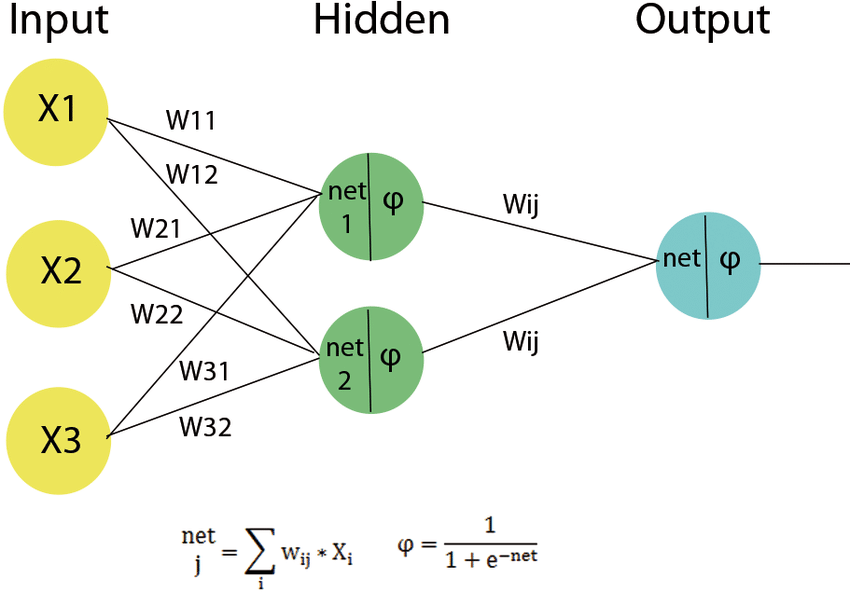
\includegraphics[width=0.7\textwidth]{rc/equation.png}
    \caption{Neural Network Architecture\cite{Gerlitz2015Large-scaleApproach}}
    \label{fig:nn_diagram}
\end{figure}


\subsection{Graph Neural Networks}
Graph Neural Network is a branch of Neural Networks and \acrshort{gnn} is more suitable than traditional neural networks in certain graph-structured data sets. Unlike neural networks \acrshort{gnn} preserve locality because the information is shared only with its neighbours in \hyperref[sec:gshiftedsignals]{graph signals}

\subsection{Graph Representation of \acrshort{opf} Problem}
A Graph is defined as G(V, E) where V is the set of Vertices/Nodes and E is the set of edges.
As discussed in \hyperref[sec:opfIdentify]{Problem Identification} the nodes of the graph of this \acrshort{opf} problem can be represented as follows,\cite{Owerko2020OptimalNetworks}

\[
 \begin{array}{l}
x^{( i)} \ =\ \left[ v^{( i)} \ \delta ^{( i)} \ p^{( i)} \ q^{( i)}\right]
\end{array}
\]

\[
 \begin{array}{l}
 X^{N*4}
\end{array}
\]

The edges of the graph are represented by the transmission lines and the weights of the edges can be represented by the following weight matrix.

\[W^{(N*N)}\]

where each element of the matrix is calculated by following equation. Here $z_{(i,j)}$ is the impedance of the power line connecting nodes i and j and k is a scaling factor,

\[w_{(i,j)} = e^{-k{\mid z_{(i,j)} \mid}^2}\]

\subsection{Graph Shifted Signals}
\label{sec:gshiftedsignals}
A k shifted graph signal can be obtained by multiplying the weight matrix k times, by the previously defined input matrix X as follows\cite{Owerko2020OptimalNetworks},

\[X_{k\ shifted} = W^{k} . X\]
\\In a single shifted graph signal $f^{th}$ feature of $i^{th}$ node is shown by the linear combination of the $f^{th}$ feature of its neighbouring nodes and weights between $i^{th}$ node and the neighbouring nodes. $N(j)$ is the number of neighbours of $j^th$ node. 
\[x_{single\ shifted\ (i)}^f = \sum_{j=1}^{N(j)} = w_{(i,j)} * x_j^f\]
As an example, shifted signal of the feature voltage of $i^{th}$ node is calculated by,
\[v_{single\ shifted\ (i)} = \sum_{j=1}^{N(j)} = w_{(i,j)} * v_j\]

\subsection{Forward Propagation}
In each layer of the Neural Network, we generate K shifted graph signals, $$X,WX,W^{2}X,..,W^{k}X$$. Then we multiply each of these shifted graph signals with the relevant coefficient matrices of $l^{th}$ layer as shown in Figure \ref{fig:gnn_diagram} \cite{Owerko2020OptimalNetworks}. $K_l$ is the number of shifts in $K^{th}$ layer and $H_{lk}$ is the coefficient matrix of $k^{th}$ shifted signal of $l^{th}$ layer.
\begin{figure}[H]
    \centering
    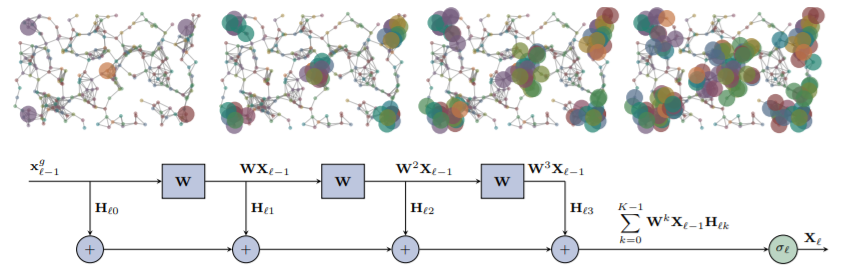
\includegraphics[width=1\textwidth]{rc/Owerko_GNN.png}
    \caption{Graph Neural Network Architecture\cite{Owerko2020OptimalNetworks}}
    \label{fig:gnn_diagram}
\end{figure}
Then we calculate linear combinations of shifted graph signals and their corresponding coefficient matrices.

\[\sum_{k=0}^{K_l-1} W^{k} . X . H_{lk}\]

Then the results is passed through a non linear activation function to obtain the value of the output of the node at $l^{th}$ layer,

\[ \sigma( \sum_{k=0}^{K_l-1} W^{k} . X . H_{lk}) \]


\subsection{\acrshort{opf} Problem Using \acrshort{gnn} Model}
The proposed model for the solution of \acrshort{opf} problem using \acrshort{gnn} is shown in the Figure \ref{fig:model}. The network is represented by the admittance matrix and load demand of each bus is given to the model as the input. The Graph Neural Network Model calculate the real-time Power Generation needed to reduce the total cost.\\


\begin{figure}[H]
    \centering
    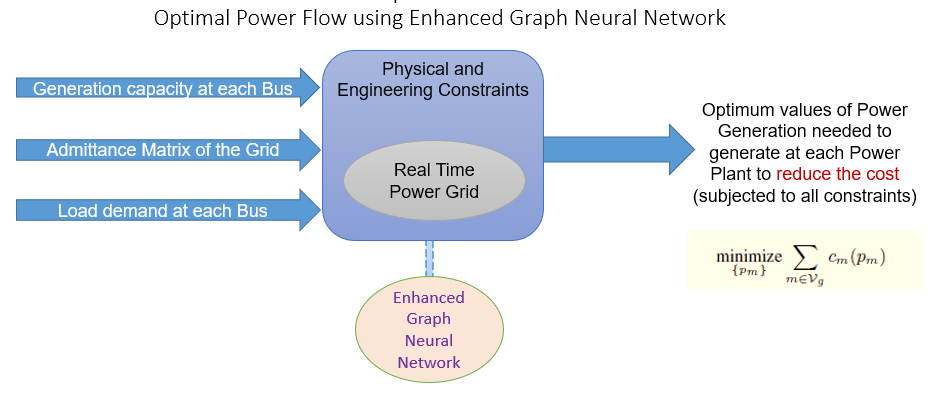
\includegraphics[width=1\textwidth]{Images/Model.PNG}
    \caption{Model for \acrshort{gnn} based \acrshort{opf} Problem }
    \label{fig:model}
\end{figure}

\section{Experiments}
\subsection{Software and Packages Used}

Following software packages are used in this project.
\begin{itemize}
    \item Google Colab Figure \ref{fig:colab}
    \item PandaPower \cite{Thurner2017PandapowerSystems} Figure \ref{fig:panda}
    \item The Graph Neural Network Library F. Gama
    \item Skorch,Sklearn,Numpy Python Libraries
\end{itemize}

\begin{figure}[H]
    \centering
    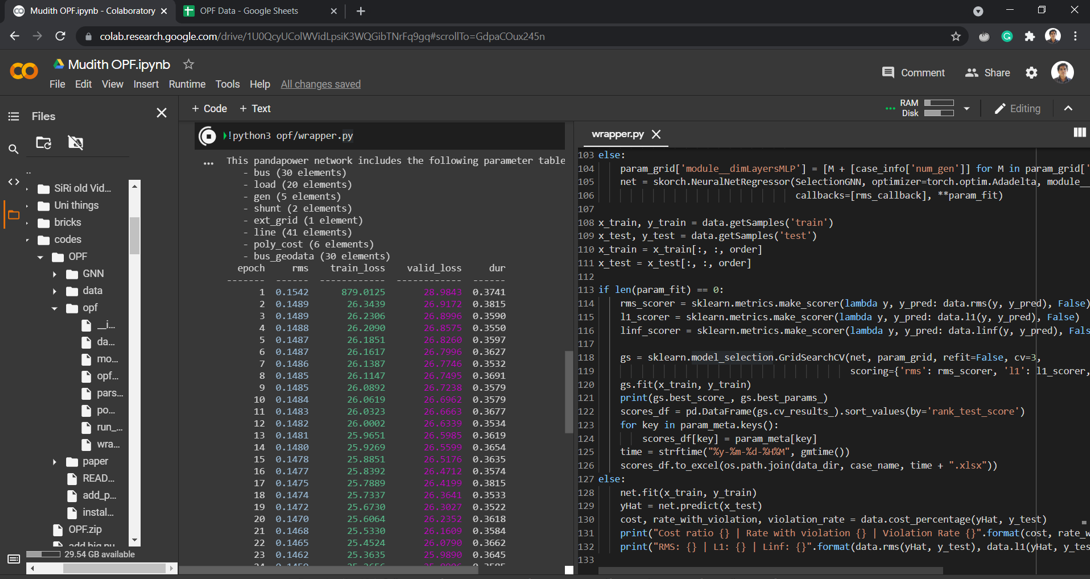
\includegraphics[width=0.8\textwidth]{Images/Colab.PNG}
    \caption{Running the codes in Google Colab Interface }
    \label{fig:colab}
\end{figure}

\begin{figure}[H]
    \centering
    
\includegraphics[width=0.8\textwidth]{Images/pandapower.PNG}
    \caption{Panda Power Documentation }
    \label{fig:panda}
\end{figure}

\subsection{Data Sets and Codes}
Test data was generated using the IEEE 30 test case which was  accessed using Pandapower\cite{Thurner2017PandapowerSystems}.
The figure \ref{fig:case30} shows a schematic diagram of IEEE 30 test case.

\begin{figure}[H]
    \centering
    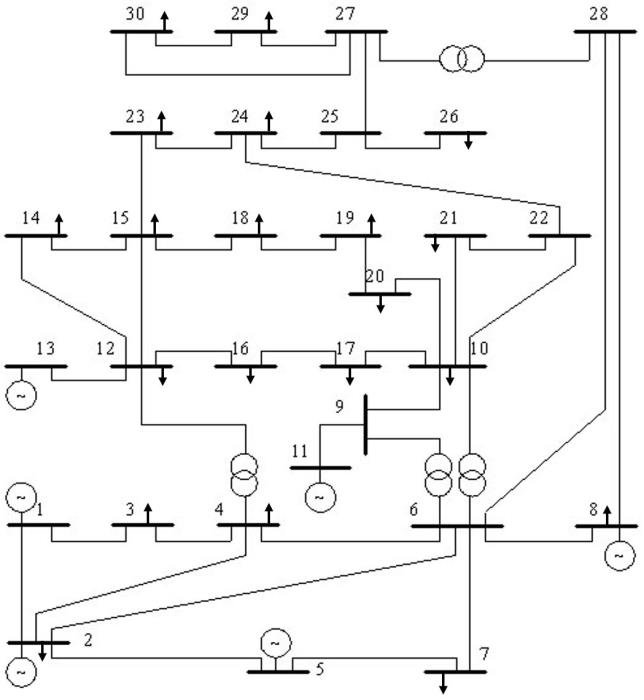
\includegraphics[width=0.5\textwidth]{Images/case30}
    \caption{Diagram of IEEE 30 Bus test Case \cite{Mohammadi2017AllocationCost}}
    \label{fig:case30}
\end{figure}

Pandapower Package has inbuilt objects that store these networks and they are easily accessible using one line of code as shown in Figure \ref{fig:panda2}. Thus the internal structure of IEEE 30 case was not analysed in this project.

\begin{figure}[H]
    \centering
    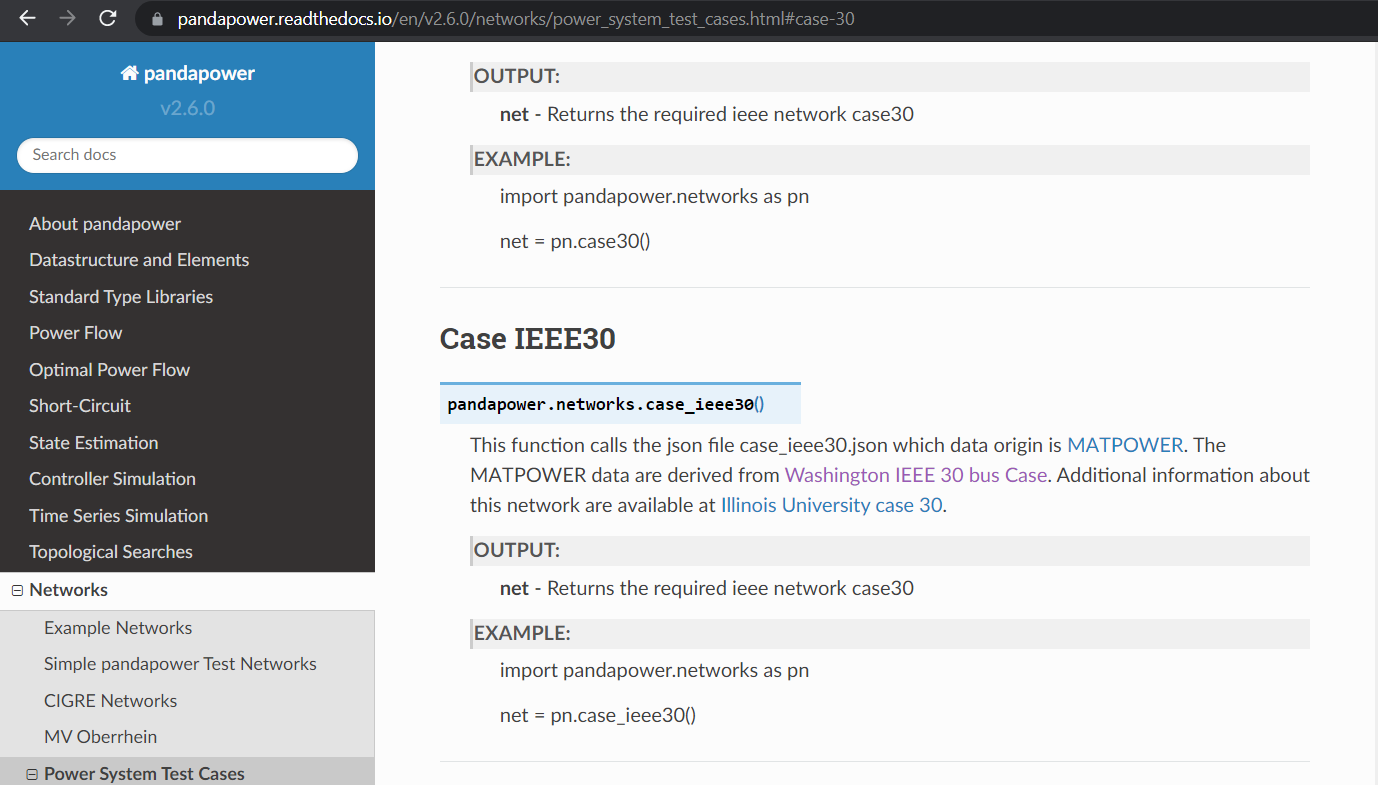
\includegraphics[width=1\textwidth]{Images/pandapower2.PNG}
    \caption{Accessing IEEE 30 test case using Panda Power }
    \label{fig:panda2}
\end{figure}

These networks are loaded using the Python codes shown in Figure \ref{fig:load} below.

\begin{figure}[H]
    \centering
    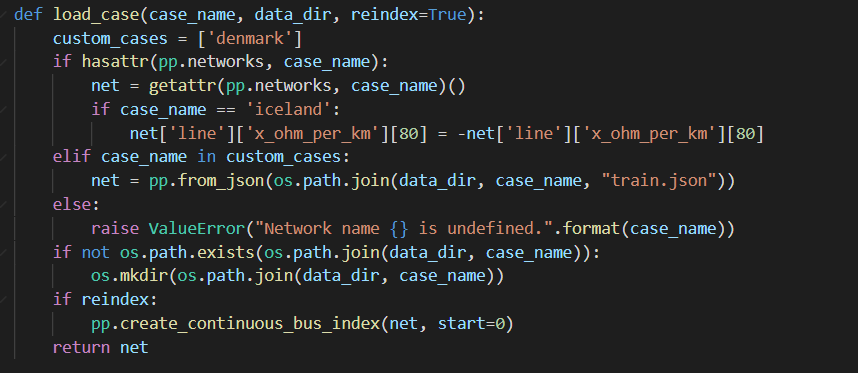
\includegraphics[width=1\textwidth]{Images/LoadCase.PNG}
    \caption{Loading the test cases }
    \label{fig:load}
\end{figure}

A large dataset is needed to train our \acrshort{gnn} model and this dataset was generated from a uniform distribution of each test case. The Python code used to generate these data\cite{Owerko2020OptimalNetworks} from a uniform distribution is shown below in Figure \ref{fig:uniform}.
\begin{figure}[H]
    \centering
    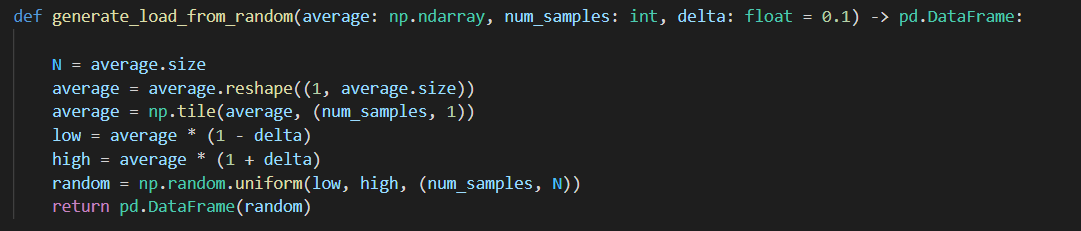
\includegraphics[width=1\textwidth]{Images/uniform.PNG}
    \caption{Generating test data from a uniform distribution}
    \label{fig:uniform}
\end{figure}

In addition, Numpy, Pytorch, Sklearn(Figure \ref{fig:sklearn}) and Skorch(Figure \ref{fig:skorch}) libraries are used in codes.

\begin{figure}[H]
    \centering
    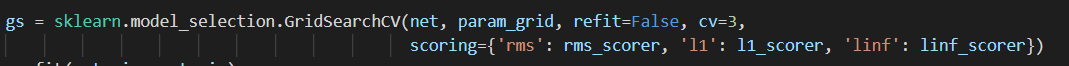
\includegraphics[width=1\textwidth]{Images/sklearn.PNG}
    \caption{Using sklearn Library}
    \label{fig:sklearn}
\end{figure}

\begin{figure}[H]
    \centering
    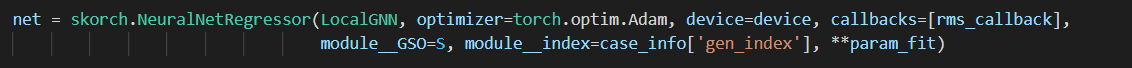
\includegraphics[width=1\textwidth]{Images/skorch.PNG}
    \caption{Using skorch Library}
    \label{fig:skorch}
\end{figure}

The localGNN in Figure \ref{fig:skorch} is a class developed by D.Owerko and F.Gama \cite{Owerko2020OptimalNetworks} in order to use the skorch library(a general Neural Network Library) for Graph Neural Networks.
\subsection{Evaluation Criteria }

We are using two Error Functions commonly used in Neural Network, RMS Error and L1 error. \\

RMS Error defined below is the root mean squared error between the predicted values and the true values. The predicted values are obtained using the graph neural network model and true values are obtained using Interior Point Optimization(IPOPT) method in Pandapower\cite{Thurner2017PandapowerSystems}. Here $n$ denotes the number of test cases.

$$RMS\ Error = \sqrt{(\frac{1}{n})\sum_{i=1}^{n}(y^{predicted}_{i} - y^{True}_{i})^{2}}$$
L1 Error or the Mean Absolute Error is defined as follows. It is calculated as the mean of the absolute values of predicted values and the true values. True values are calculated from the Interior Point Optimization(IPOPT) Method from Pandapower\cite{Thurner2017PandapowerSystems}.

$$L1\ Error (Mean\ Absolute\ Error) = (\frac{1}{n})\sum_{i=1}^{n}\left | y^{predicted}_{i} - y^{True}_{i} \right |$$
The Figure \ref{fig:rmsl1} shows the functions used to calculate these error values.
\begin{figure}[H]
    \centering
    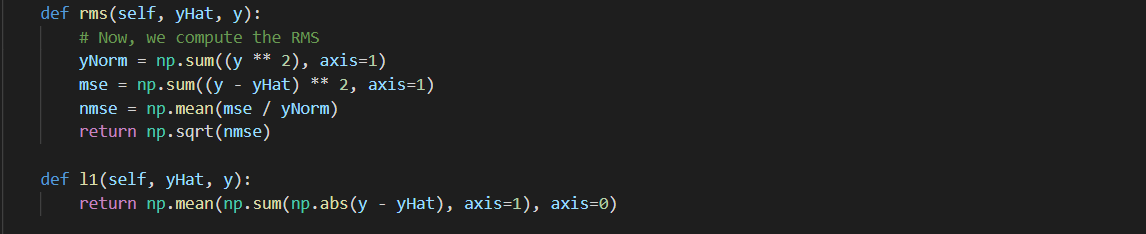
\includegraphics[width=1\textwidth]{Images/rmsl1.PNG}
    \caption{Functions used to Calculate RMS Error and L1 Error}
    \label{fig:rmsl1}
\end{figure}


\subsection{Changing Parameters of the Model}

I experimented with this \acrshort{gnn} based \acrshort{opf} solution by changing the parameters such as number of features in each layer, number of filter taps, etc.

An example code of experimenting with parameters is shown below in Figure \ref{fig:param}.
\begin{figure}[H]
    \centering
    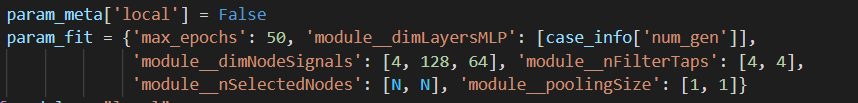
\includegraphics[width=1\textwidth]{Images/param_fit.PNG}
    \caption{Experimenting with Different Parameters}
    \label{fig:param}
\end{figure}

\newpage
\subsection{Selection vs Local \acrshort{gnn} }

Both Selection GNN and Local GNN consist of graph convolution layers and one readout layer. But the readout layer of Selection GNN Architecture has separate values in each node which is the amount of power that needs to be generated at each node(bus). \\

In Global GNN Architecture, the final layer is fully connected and it has M(Number of Generators) number of outputs.

\section{Results}

\subsection{Architecture}

Here, I did experiments with the number of features in each layer and obtained the results shown in Figure \ref{fig:architecture}. I have omitted the number of features in the input layer and the output layer since they are pre-defined. 

The results are obtained after fixing the optimizer to Ada delta and other parameters to default values. Default values are highlighted in yellow in each table.

\begin{figure}[H]
    \centering
    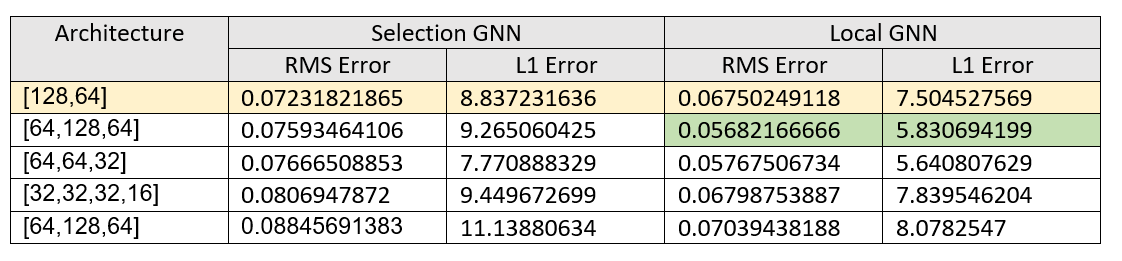
\includegraphics[width=1\textwidth]{Images/Architecture.PNG}
    \caption{Experiments with \acrshort{gnn} Architecture}
    \label{fig:architecture}
\end{figure}

\subsection{Optimizer} 

The Figure \ref{fig:optimizer} shows the results for different optimizers fixing Architecture, Scaling Factor, Threshold and Filter Taps to constant values.
\begin{figure}[H]
    \centering
    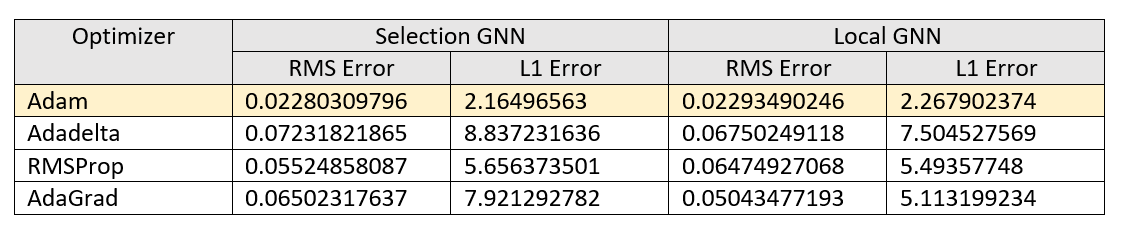
\includegraphics[width=1\textwidth]{Images/Optimizer.PNG}
    \caption{Experiments with Optimizer}
    \label{fig:optimizer}
\end{figure}

\newpage

\subsection{Scaling Factor} 
The scaling factor is the value of $k$ in the equation we have used to calculate the weight in the admittance matrix. The equation is shown below. Larger $k$ values reduce the weights(which represents admittances) in exponential factors. 
\[w_{(i,j)} = e^{-k{\mid z_{(i,j)} \mid}^2}\]

The experiment results for different scaling factors are shown in figure \ref{fig:scaling_factor}.
\begin{figure}[H]
    \centering
    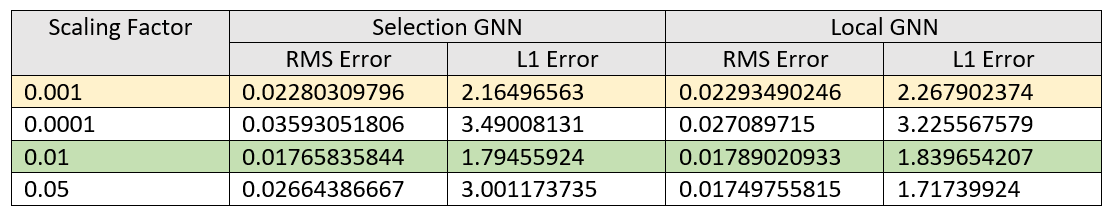
\includegraphics[width=1\textwidth]{Images/Scaling_Factor.PNG}
    \caption{Experiments with Scaling Factor}
    \label{fig:scaling_factor}
\end{figure}

\subsection{Threshold} 
The weights in the admittance matrix, below the threshold, are redefined to zero. These weights represent the buses that are far away from each other and neglecting their interconnection can improve the calculation speed while increasing accuracy.
The experiment results for two threshold values are shown in figure \ref{fig:threshold}.
\begin{figure}[H]
    \centering
    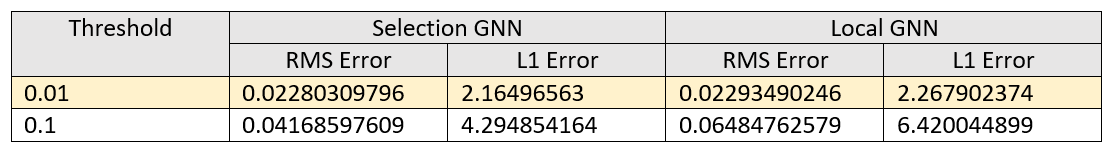
\includegraphics[width=1\textwidth]{Images/Thresshold.PNG}
    \caption{Experiments with Threshold}
    \label{fig:threshold}
\end{figure}

\subsection{Filter Taps} 
Filter taps are defined as the number of graph convolutions done in each internal layer. K number of filter taps implies an exchange of values with the k-hop neighbourhood in the graph.
Experiment results for different filter taps are shown in figure \ref{fig:Filter Taps}.
\begin{figure}[H]
    \centering
    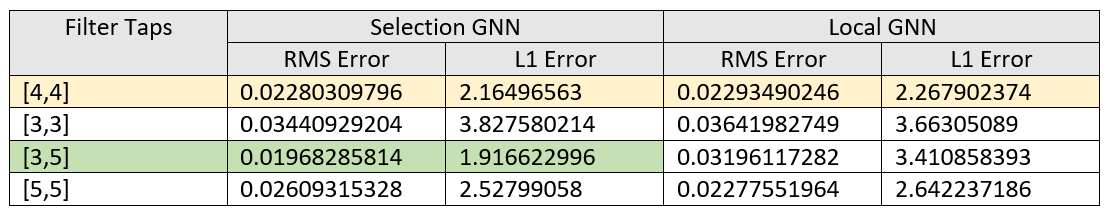
\includegraphics[width=1\textwidth]{Images/Filter_Taps.PNG}
    \caption{Experiments with Filter Taps}
    \label{fig:Filter Taps}
\end{figure}

\newpage

\section{Conclusion and Further Improvements}

This project shows that changing number of features in each layer,filter taps in each layer and specially scaling factor significantly improve the accuracy of optimal power flow solution. The rows highlighted in green in the Figures \ref{fig:architecture}  \ref{fig:scaling_factor} \ref{fig:Filter Taps} depicts these improvements.
But changing the optimizer does not improve the overall accuracy significantly and Adam optimizer which is the default choice in the work\cite{Owerko2020OptimalNetworks} is proven to be the best optimizer in neural network propagation.\\

The [64,128,64] architecture experimented(shown in green in Figure \ref{fig:architecture}) has outperformed other architectures for local GNN. In this architecture, the number of features is maximum in the middle layer and it gradually decrease towards input and output layers.\\

The best improvement was gained from the scaling factor. As shown in Figure \ref{fig:scaling_factor} 0.01 scale factor has outperformed the 0.001 scaling factor by a significant margin. The improvement of RMS Error is $29.54\%$ for the selection GNN. The meaning of using 0.01 instead of 0.001 is taking the $10^{th}$ power of previous weights. This in turn further reduces small weights while exaggerating larger weights. Here weight resemble the admittance. \\

Changing the threshold has no improvement on error values and thus we conclude the best threshold is 0.01,which is the default value used in work \cite{Owerko2020OptimalNetworks}.\\

In Filter Taps, results shown in figure \ref{fig:Filter Taps} [3,5] configuration has outperformed default filter tap values of [4,4] for selection GNN. This new filter tap configuration has three graph convolutions in the first inner layer and five graph convolutions in the second inner layer. This enables the model to share data only with 3-hop neighbours in the first inner layer and then share with the 5-hop neighbourhood in the next inner layer. I assume this method is better since it gives priority to close neighbours in initial information sharing.\\
 
There are many paths to extend this work. It is possible to include constraints in the power system such as the maximum currents that can pass through each transmission line. In addition, the security-constrained optimal power flow problem is a branch of \acrshort{opf} problem. It finds a solution that will continue working under the failure of one or more power plants. Someone can attempt to solve these problems as well using Graph Neural Networks.\\

Since the change in the scaling factor brought the highest improvement I suggest that there can be a better mathematical function for the weights in the admittance matrix.\\

Furthermore, novel trends in Deep Neural Networks and Artificial Intelligence such as Residual Neural Networks(RESNET)\cite{He2016DeepRecognition} can also be applied to this \acrshort{gnn} based \acrshort{opf} problem.\\



\newpage

\bibliographystyle{IEEEtran}
\bibliography{references}


\end{document}